\documentclass{beamer}
\let\Tiny=\tiny %to avoid warnings related to font size and beamer 
\usetheme{Amsterdam}
\usecolortheme{dolphin}
\usepackage{color}
\usepackage{amsmath}
\usepackage{tikz}
\usepackage{verbatim}
\usetikzlibrary{arrows,shapes}
\usepackage{hyperref}
\usepackage[style=verbose,backend=bibtex]{biblatex}
\usepackage{comment}
\usepackage{listings}
\usepackage{algorithm}
\usepackage{algpseudocode}
%\usepackage{color}

\addbibresource{../sources}

\definecolor{OliveGreen}{cmyk}{0.64,0,0.95,0.40}

\let\oldfootnotesize\footnotesize
\renewcommand*{\footnotesize}{\oldfootnotesize\tiny}

\title{Parallel network flows}
\subtitle{A follow up seminar to the Parallel Algorithms lecture}
\author{Martin Kalany\inst{1} }
\institute
{
  \inst{1}
  Graduate student in Computer Science\\
  Vienna University of Technology\\
}
\date{\today}

\AtBeginSection[]
{
  \begin{frame}
    \frametitle{Table of Contents}
    \tableofcontents[currentsection]
  \end{frame}
}

\tikzstyle{vertex}=[circle,fill=black!25,minimum size=20pt,inner sep=0pt]
\tikzstyle{edge} = [draw,thick,->,>=latex,shorten >=1pt]
\tikzstyle{weight} = [font=\small]
\tikzstyle{selected edge} = [draw,line width=2pt,->,red!75,>=latex]
\tikzstyle{residual edge} = [draw,thick,->,blue!75,>=latex]
\tikzstyle{vertexE}=[circle,fill=black!25,minimum size=20pt,inner sep=0pt]


\begin{document}
% Declare layers (for more convenience when drawing graphs)
\pgfdeclarelayer{background}
\pgfsetlayers{background,main}

\frame{\titlepage}
	
\section{Network flows}
\begin{frame}
	\frametitle{Network flows}
    \begin{block}{Definition: Flow network}\footnote{\cite{ahuja93}}
    A \textcolor{red}{flow network}  is given by $N = (G,s,t,c)$, where
    \begin{itemize}
    		\item $G =(V,A)$ is a directed graph
    		\item $s$ and $t$, $s \neq t$ are the source and terminal node
    		\item $c:A\rightarrow \mathbb{R}_0^{+}$ assigns a capacity $\forall a \in A$
    \end{itemize}
    \end{block}
    \textbf{Assumptions:}
	\begin{itemize}
		\item $G$ is connected
		\item $\nexists P(s,t) \in G$ s.t. $c(P) = \infty$
		\item $G$ is simple, i.e., does not contain loops or parallel arcs
	\end{itemize}
\end{frame}
  
\begin{frame}[shrink]
	\frametitle{Network flows}
	\begin{block}{Definition: Flow}
	$f:A \rightarrow \mathbb{R}_0^{+}$ is a \textcolor{red}{flow} if it satisfies:
	\begin{itemize}
		\item \textbf{Capacity constraints:} $f(a) \leq c(a)$ $\forall a \in A$
		\item \textbf{Flow conservation:} 
		$ \sum\limits_{v \in V} f(u,v) =  0 \Leftrightarrow IN(f,v) = OUT(f,v)$ $\forall v \in V \setminus \{s,t\}$
		\item \textbf{Value of a flow:} $\lvert f\rvert = f(V,t)$ 
	\end{itemize}
	\end{block}
	
	\begin{block}{A flow $f$}
	\begin{itemize}
		\item is a \textcolor{red}{maximum flow} if $\lvert f\rvert \geq \lvert f'\rvert$, for any other flow $f'$
		\item \textcolor{red}{saturates} an arc a if $f(a) = c(a)$
		\item is a \textcolor{red}{maximal (or blocking) flow} if every directed path P(s,t) contains at least one saturated edge
	\end{itemize}
	\end{block}
\end{frame}

\begin{frame}
	\frametitle{Network flows}
	\begin{block}{Definition: Residual capacity}
		The \textcolor{red}{residual capacity} of $a \in V \times V$ w.r.t. a flow $f$ is defined as $r_f(a) = c(a) - f(a)$. \\
	\end{block}
	
	\pause
	\begin{block}{Definition: Residual network}
		$G_r = (V, A_r)$ with $A_r = \left\{a \in V \times V \lvert r_f(a) > 0\right\}$
	\end{block}
	
	\pause
	\begin{block}{Definition: Augmenting path}
		A path $P$ from $s$ to $t$ in $G_r$ is called an \textcolor{red}{augmenting} path and can be used to increase the flow $f$.
	\end{block}
\end{frame}

%\section{Ford-Fulkerson}
\begin{frame}
	\frametitle{Algorithm of Ford-Fulkerson}
	\framesubtitle{An intuitive sequential algorithm}
	
	\visible<1-2>{
	\begin{figure}
	\begin{tikzpicture}[scale=1.8, auto,swap]
    	% draw the vertices
	    \foreach \pos/\name in {{(0,2)/s}, {(1,3)/v_1}, {(2.5,3)/v_2},
    	                        {(1,1)/v_3}, {(2.5,1)/v_4}, {(3.5,2)/t}}
        \node[vertex] (\name) at \pos {$\name$};
    	% Connect vertices with edges and draw weights
    	\foreach \source/ \dest /\weight in {s/v_1/2, s/v_3/8,v_3/v_1/5,
                                         v_1/v_2/7, v_4/v_2/15, v_3/v_4/5,
                                         v_2/t/2, v_4/t/5}
        	\path[edge] (\source) -- node[weight] {$\weight$} (\dest);
        	
        	%v_1/v_4/9
        	\path[edge] ([xshift= -2pt, yshift= 5pt] v_4.center) -- node[weight] {6}  ([xshift= 5pt, yshift= -2pt] v_1.center);
        	\path[edge] ([xshift = 2pt, yshift= -5pt] v_1.center) -- node[weight] {9}  ([xshift= -5pt, yshift= 2pt] v_4.center);
  
	    % For convenience we use a background layer to highlight edges
    	% This way we don't have to worry about the highlighting covering
	    % weight labels. 
	    \begin{pgfonlayer}{background}
	        \pause
    	    \foreach \source /\dest  /\weight in {s/v_3/5,v_4/t/5}
	            \path[selected edge] (\source) -- node[weight,above] {$\weight$}(\dest);		
	            \path[selected edge] ([xshift = 2pt, yshift= -5pt] v_1.center) -- node[weight,left] {5}  ([xshift= -5pt, yshift= 2pt] v_4.center);
	            \path[selected edge] (v_3) -- node[weight,left] {$5$}(v_1);
    	\end{pgfonlayer}
	\end{tikzpicture}
	\end{figure}
	}	
\end{frame}

\begin{frame}
	\frametitle{Algorithm of Ford-Fulkerson}
	\framesubtitle{An intuitive sequential algorithm}

	\begin{figure}
	\begin{tikzpicture}[scale=1.8, auto,swap]
    	% draw the vertices
	    \foreach \pos/\name in {{(0,2)/s}, {(1,3)/v_1}, {(2.5,3)/v_2},
    	                        {(1,1)/v_3}, {(2.5,1)/v_4}, {(3.5,2)/t}}
        \node[vertex] (\name) at \pos {$\name$};
    	% Connect vertices with edges and draw weights
    	\foreach \source/ \dest /\weight in {s/v_1/2, v_1/v_3/5, t/v_4/5,
                                         v_1/v_2/7, v_4/v_2/15, v_3/v_4/5,
                                         v_2/t/2}
        	\path[residual edge] (\source) -- node[weight] {$\weight$} (\dest);

        	%s/v_3/8,
        	\path[residual edge] ([xshift= -2pt, yshift= 5pt] v_3.center) -- node[weight] {5}  ([xshift= 5pt, yshift= -2pt] s.center);
        	\path[residual edge] ([xshift = 2pt, yshift= -5pt] s.center) -- node[weight] {3}  ([xshift= -5pt, yshift= 2pt] v_3.center);
        	%v_1/v_4/9
        	\path[residual edge] ([xshift= -2pt, yshift= 5pt] v_4.center) -- node[weight] {11}  ([xshift= 5pt, yshift= -2pt] v_1.center);
        	\path[residual edge] ([xshift = 2pt, yshift= -5pt] v_1.center) -- node[weight] {4}  ([xshift= -5pt, yshift= 2pt] v_4.center);       	
        	
        	\begin{pgfonlayer}{background}
	        \pause
    	    \foreach \source /\dest  /\weight in {s/v_1/2,v_1/v_2/2,v_2/t/2}
	            \path[selected edge] (\source) -- node[weight,above] {$\weight$}(\dest);			            
    	\end{pgfonlayer}
	\end{tikzpicture}
	\end{figure}	
\end{frame}		

\begin{frame}
	\frametitle{Algorithm of Ford-Fulkerson}
	\framesubtitle{An intuitive sequential algorithm}

	\begin{figure}
	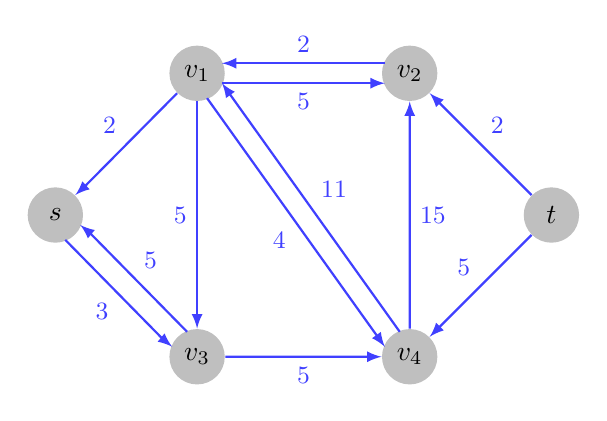
\begin{tikzpicture}[scale=1.8, auto,swap]
    	% draw the vertices
	    \foreach \pos/\name in {{(0,2)/s}, {(1,3)/v_1}, {(2.5,3)/v_2},
    	                        {(1,1)/v_3}, {(2.5,1)/v_4}, {(3.5,2)/t}}
        \node[vertex] (\name) at \pos {$\name$};
    	% Connect vertices with edges and draw weights
    	\foreach \source/ \dest /\weight in {v_1/s/2, v_1/v_3/5, t/v_4/5,
                                         v_4/v_2/15, v_3/v_4/5,
                                         t/v_2/2}
        	\path[residual edge] (\source) -- node[weight] {$\weight$} (\dest);

        	%s/v_3/8,
        	\path[residual edge] ([xshift= -2pt, yshift= 5pt] v_3.center) -- node[weight] {5}  ([xshift= 5pt, yshift= -2pt] s.center);
        	\path[residual edge] ([xshift = 2pt, yshift= -5pt] s.center) -- node[weight] {3}  ([xshift= -5pt, yshift= 2pt] v_3.center);
        	%v_1/v_4/9
        	\path[residual edge] ([xshift= -2pt, yshift= 5pt] v_4.center) -- node[weight] {11}  ([xshift= 5pt, yshift= -2pt] v_1.center);
        	\path[residual edge] ([xshift = 2pt, yshift= -5pt] v_1.center) -- node[weight] {4}  ([xshift= -5pt, yshift= 2pt] v_4.center);       	
			%v_1/v_2/7
        	\path[residual edge] ([xshift= 5pt, yshift= -2pt] v_1.center) -- node[weight] {5}  ([xshift= -5pt, yshift= -2pt] v_2.center);
        	\path[residual edge] ([xshift = -5pt, yshift= 2pt] v_2.center) -- node[weight] {2}  ([xshift= 5pt, yshift= 2pt] v_1.center);               		
	\end{tikzpicture}
	\end{figure}
\end{frame}		

\begin{frame}
	\frametitle{Algorithm of Ford-Fulkerson}
	\framesubtitle{An intuitive sequential algorithm}
	
	\begin{columns}[c] 
    \column{.5\textwidth} 
	\begin{figure}
	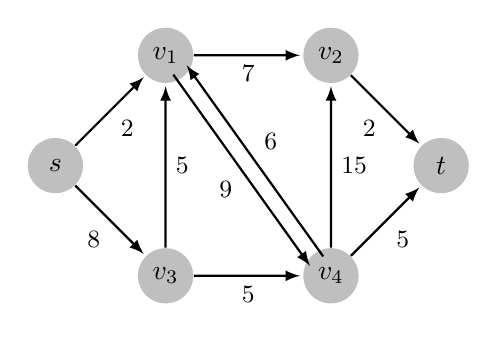
\begin{tikzpicture}[scale=1.4, auto,swap]
    	% draw the vertices
	    \foreach \pos/\name in {{(0,2)/s}, {(1,3)/v_1}, {(2.5,3)/v_2},
    	                        {(1,1)/v_3}, {(2.5,1)/v_4}, {(3.5,2)/t}}
        \node[vertex] (\name) at \pos {$\name$};
    	% Connect vertices with edges and draw weights
    	\foreach \source/ \dest /\weight in {s/v_1/2, s/v_3/8,v_3/v_1/5,
                                         v_1/v_2/7, v_4/v_2/15, v_3/v_4/5,
                                         v_2/t/2, v_4/t/5}
        	\path[edge] (\source) -- node[weight] {$\weight$} (\dest);
        	
        	%v_1/v_4/9
        	\path[edge] ([xshift= -2pt, yshift= 5pt] v_4.center) -- node[weight] {6}  ([xshift= 5pt, yshift= -2pt] v_1.center);
        	\path[edge] ([xshift = 2pt, yshift= -5pt] v_1.center) -- node[weight] {9}  ([xshift= -5pt, yshift= 2pt] v_4.center);	 
	\end{tikzpicture}
	\end{figure}
    \column{.5\textwidth}
	\begin{figure}
	\begin{tikzpicture}[scale=1.4, auto,swap]
    	% draw the vertices
	    \foreach \pos/\name in {{(0,2)/s}, {(1,3)/v_1}, {(2.5,3)/v_2},
    	                        {(1,1)/v_3}, {(2.5,1)/v_4}, {(3.5,2)/t}}
        \node[vertex] (\name) at \pos {$\name$};
    	
	    \begin{pgfonlayer}{background}
    	    \foreach \source /\dest  /\weight in {s/v_3/5,v_4/t/5,s/v_1/2,v_1/v_2/2,v_2/t/2}
	            \path[selected edge] (\source) -- node[weight,above] {$\weight$}(\dest);		
	            \path[selected edge] ([xshift = 2pt, yshift= -5pt] v_1.center) -- node[weight,left] {5}  ([xshift= -5pt, yshift= 2pt] v_4.center);
	            \path[selected edge] (v_3) -- node[weight,left] {$5$}(v_1);
    	\end{pgfonlayer}
	\end{tikzpicture}
	\end{figure}
    \end{columns}	
\end{frame}

\section{Computational Complexity}
\begin{frame}
	\frametitle{Computational Complexity}
	\begin{itemize}
		\item Sequential complexity:
		\begin{itemize}
			\item Ford-Fulkerson: $O((|A|+|V|)*f_{max})$
			\item Edmonds-Karp: $O(|V|^{2} * |E|) $
			\pause \\	
			$\Rightarrow$ \textcolor{green}{clearly solvable in polynomial time}
		\end{itemize}
		\pause
		\item Parallel complexity:
		\begin{itemize}
			\item Construct residual network: $O(1)$
			\item Find augmenting path: $O(log^{2}|V|)$ time and $O(|V|^{2})$ work
			\item Number of stages: $O(|f_{max}|)$\\
			may be reduced\footcite{papa95} to $O(|V|)$ or even $O(\sqrt{|V|})$
		\end{itemize}			
		\pause
		\textcolor{blue}{Can we get an "efficient" parallel algorithm?}
	\end{itemize}
\end{frame}

\begin{frame}
	\frametitle{Computational Complexity}
	\begin{itemize}
	\item \textbf{NC}\footcite{papa95} ("Nick's Class"): Problems solvable in $O(log^{k_1}(n))$ time and $O(n^{k_2})$ total work
	\item alternatively: Language decided by PRAM in $O(log^{k_1}(n))$ time steps with $O(n^{k_2})$ processors available at each step 
	\item $NC \subseteq P$, but whether $NC \subset P$ or $NC = P$ is unknown 
	\item $P \setminus NC$: "Inherently sequential"  problems
	\item Most likely candidates to be in $P \setminus NC$: P-complete problems
	\end{itemize}

	\pause	
	\textcolor{red}{Max-flow is P-complete.} \\
	No parallel algorithm to solve the problem in poly-log time is currently known.	
\end{frame}

\section{Shiloach-Vishkin}
\begin{frame}
\frametitle{Layered networks}
	\begin{block}{Definition: Layered network\footcite{yossi81}}
	$N = (V,A,s,t,c)$ is a \textcolor{red}{layered network} if each vertex $v \in V$ has a layer number $l(v)$ s.t.
	\begin{itemize}
		\item $l(s) = 0$ and $0 \leq l(v) \leq l(t)$ $\forall v \in V$
		\item $(e = u \rightarrow v) \in A  \Rightarrow l(v) - l(u) = 1$
	\end{itemize}
	\end{block}
\end{frame}

\begin{frame}
\frametitle{Dinitz' scheme}	
	\begin{block}{Lemma: Dinitz' scheme\footcite{dinitz70}}
	A maximum flow problem in a \emph{general network} can be transformed \emph{into $O(n)$ maximal flow problems in layered networks}.
	\end{block}
	
	\begin{figure}
	\begin{tikzpicture}[scale=1.2, auto,swap]
    	% draw the vertices
	    \foreach \pos/\name/\layer in {{(0,2)/s/0}, {(1,3)/v_1/1}, {(2.5,3)/v_2/2},
    	                        {(1,1)/v_3/1}, {(2.5,1)/v_4/2}, {(3.5,2)/t/3}}
        \node[vertex,label={[color=blue]80:$\layer$}] (\name) at \pos {$\name$};
        
        %\node[vertex,label={[color=blue]80:$+12$}] (v_1) at (1.5,3) {$v_1$};
    	% Connect vertices with edges and draw weights
    	\foreach \source/ \dest in {s/v_1, s/v_3,v_3/v_1,
                                         v_1/v_2, v_4/v_2, v_3/v_4,
                                         v_2/t, v_4/t}
        	\path[edge] (\source) -- (\dest);
        	
        	%v_1/v_4/9
        	\path[edge] ([xshift= -2pt, yshift= 5pt] v_4.center) -- ([xshift= 5pt, yshift= -2pt] v_1.center);
        	\path[edge] ([xshift = 2pt, yshift= -5pt] v_1.center) -- ([xshift= -5pt, yshift= 2pt] v_4.center);
  
	    % For convenience we use a background layer to highlight edges
    	% This way we don't have to worry about the highlighting covering
	    % weight labels. 
	    \begin{pgfonlayer}{background}
    	    \foreach \source /\dest in {s/v_3,v_2/t,s/v_1,v_1/v_2,v_3/v_4,v_4/t}
	            \path[selected edge, color=blue] (\source) -- (\dest);		
	            \path[selected edge, color=blue] ([xshift = 2pt, yshift= -5pt] v_1.center) -- ([xshift= -5pt, yshift= 2pt] v_4.center);
	    \end{pgfonlayer}
	\end{tikzpicture}
	\end{figure}
\end{frame}

\begin{frame}
\frametitle{Algorithm 1: Shiloach and Vishkin\footcite{yossi81}}
\framesubtitle{High level description}
	\begin{algorithmic}[1]
	\Function{MAX-FLOW}{$N=(V,A,s,t,c)$}
	\State start with some valid flow 
	\While{$l(t) \neq \infty$} \Comment{\textcolor{OliveGreen}{$O(\lvert V \rvert)$}}	
		\State Construct residual network $G_r$ \Comment{\textcolor{OliveGreen}{$O(\lvert V \rvert)$, $p=O(\lvert V \rvert)$}}
		\State Construct layered network $G_l$ from $G_r$ \Comment{\textcolor{OliveGreen}}{$O(\lvert A \rvert/p + \lvert V \rvert)$}
		\State $f_l$ = MAX-FLOW($G_l$)  \Comment{next slides}
		\State $f$ = $f$ + $f_l$ \Comment{\textcolor{OliveGreen}{$O(\lvert V \rvert)$}}
	\EndWhile
	\EndFunction
	\end{algorithmic}
\end{frame}

\begin{frame}
\frametitle{Algorithm 1: Shiloach and Vishkin}
\framesubtitle{Max-Flow in a layered network}	
	\begin{algorithmic}[1]
	\Function{MAX-FLOW}{$G_l$}
		\State EXCESS(s) = $\Sigma_{v \in L_1}$ c(s$\rightarrow$v)
		\State PUSH(s, EXCESS(s))
		\State i = 1
		\While{$\exists$ v $\in$ UNBALANCED}
			\State i++
			\If{$v$ is not blocked}
				\State PUSH(v, EXCESS(v))
			\EndIf
			\State RETURN(v, EXCESS(v))
		\EndWhile
	
	\EndFunction
	\end{algorithmic}
\end{frame}

\begin{frame}[shrink]
\frametitle{Algorithm 1: Shiloach and Vishkin}
\framesubtitle{The PUSH function}
	\begin{algorithmic}[1]
	\Function{PUSH}{v, EXCESS(v)}
		\While{EXCESS(v) $>$ 0 and AVAILABLE $\neq\emptyset$}
			\State e (= v$\rightarrow$w) = first edge in AVAILABLE(v)
			\State q = min\{c(e) - f(e), EXCESS(v)\}
			\State add Q = (e,q) to STACK(w)
			\State f(e) = f(e) + q
			\State EXCESS(v) = EXCESS(v) - q
			\State EXCESS(w) = EXCESS(w) + q
			\If{f(e) == c(e)}
				\State remove e from AVAILABLE(v)
			\EndIf
		\EndWhile
	 	\If{AVAILABLE == $\emptyset$}
	 		\State block v
\State $\forall u$ s.t. $(u \rightarrow v) \in A$: delete $(u\rightarrow v)$ from AVAILABLE(u) 
	 	\EndIf
	\EndFunction
	\end{algorithmic}
\end{frame}

\begin{frame}[shrink]
\frametitle{Algorithm 1: Shiloach and Vishkin}
\framesubtitle{The RETURN function}
	\begin{algorithmic}[1]
	\Function{RETURN}{v, EXCESS(v)}
		\While{EXCESS(v) $>$ 0}
			\State let Q (= e=u$\rightarrow$v, q) be first element on in STACK(v)
			\State q' = min\{q, EXCESS(v)\}
			\State add Q = (e,q) to STACK(w)
			\State f(e) = f(e) - q'
			\State EXCESS(v) = EXCESS(v) - q'
			\State EXCESS(u) = EXCESS(u) + q
			\If{q' == q}
				\State delete Q from STACK(v)
			\Else
				\State Q = (e, q - q')
			\EndIf
		\EndWhile
	\EndFunction
	\end{algorithmic}
\end{frame}

%        \node[vertex,label={[color=blue]80:$\layer$}] (\name) at \pos {$\name$};
\begin{frame}
\frametitle{Algorithm 1: Shiloach and Vishkin}
\framesubtitle{Preflow-Push example}
\begin{figure}
	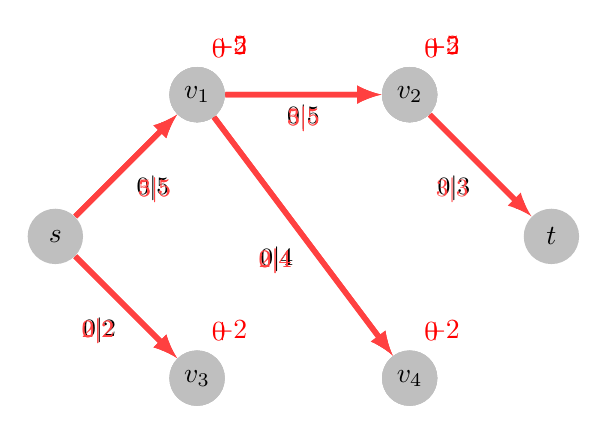
\begin{tikzpicture}[scale=1.8, auto,swap]
		% s and t don't change
	    \foreach \pos/\name in {{(0,2)/s/0},{(3.5,2)/t/0}}
       		\node[vertex] (\name) at \pos {$\name$};
       
        \foreach \pos/\name in {{(1,3)/v_1/0},{(1,1)/v_3/0}}
       		{\visible<1>{\node[vertex] (\name) at \pos {$\name$};}}
		\foreach \pos/\name in {{(2.5,3)/v_2/0}}
       		{\visible<1-2>{\node[vertex] (\name) at \pos {$\name$};}}       	
       	\foreach \pos/\name in {{(2.5,1)/v_4/0}}
       		{\visible<1->{\node[vertex] (\name) at \pos {$\name$};}}       	
       	\foreach \pos/\name/\excess in {{(1,3)/v_1/+5}}
       		{\visible<2>{\node[vertex,label={[color=red]80:$\excess$}] (\name) at \pos {$\name$};}}       	
       	\foreach \pos/\name/\excess in {{(1,1)/v_3/+2}}
       		{\visible<2>{\node[vertex,label={[color=red]80:$\excess$}] (\name) at \pos {$\name$};}}    
       	\foreach \pos/\name/\excess in {{(1,3)/v_1/0}}
       		{\visible<3-4,6,8->{\node[vertex,label={[color=red]80:$\excess$}] (\name) at \pos {$\name$};}}    
       	\foreach \pos/\name/\excess in {{(1,1)/v_3/0}}
       		{\visible<3->{\node[vertex,label={[color=red]80:$\excess$}] (\name) at \pos {$\name$};}}      	  	
       	\foreach \pos/\name/\excess in {{(2.5,3)/v_2/+5}}
       		{\visible<3>{\node[vertex,label={[color=red]80:$\excess$}] (\name) at \pos {$\name$};}}      	  	
       	\foreach \pos/\name/\excess in {{(2.5,3)/v_2/+2}}
       		{\visible<4>{\node[vertex,label={[color=red]80:$\excess$}] (\name) at \pos {$\name$};}}      	 
       	\foreach \pos/\name/\excess in {{(2.5,3)/v_2/0}}
       		{\visible<5->{\node[vertex,label={[color=red]80:$\excess$}] (\name) at \pos {$\name$};}}   
       	\foreach \pos/\name/\excess in {{(1,3)/v_1/+2}}
       		{\visible<5,7>{\node[vertex,label={[color=red]80:$\excess$}] (\name) at \pos {$\name$};}}       
       	\foreach \pos/\name/\excess in {{(2.5,1)/v_4/+2}}
       		{\visible<6>{\node[vertex,label={[color=red]80:$\excess$}] (\name) at \pos {$\name$};}}      	
       \foreach \pos/\name/\excess in {{(2.5,1)/v_4/0}}
       		{\visible<7>{\node[vertex,label={[color=red]80:$\excess$}] (\name) at \pos {$\name$};}}   	
       	
    	                      
    	% Connect vertices with edges and draw weights
	   	\foreach \source /\dest /\weight in {s/v_3/0|2,s/v_1/0|5} 
	    	{\visible<1-1>{\path[edge] (\source) --node[weight]{$\weight$} (\dest);}}
      	\foreach \source /\dest /\weight in {v_1/v_2/0|5}
	    	{\visible<1-2>{\path[edge] (\source) --node[weight]{$\weight$} (\dest);}}
	    \foreach \source /\dest /\weight in {v_1/v_4/0|4}
	    	{\visible<1-5>{\path[edge] (\source) --node[weight]{$\weight$} (\dest);}}
	   	\foreach \source /\dest /\weight in {v_2/t/0|3}
	    	{\visible<1-3>{\path[edge] (\source) --node[weight]{$\weight$} (\dest);}}	    	
    	
    	\foreach \source /\dest /\weight in {s/v_3/2|2} 
	    	{\visible<2>{\path[selected edge] (\source) --node[weight]{$\weight$} (\dest);}} 
	   \foreach \source /\dest /\weight in {s/v_1/5|5} 
	    	{\visible<2-7>{\path[selected edge] (\source) --node[weight]{$\weight$} (\dest);}}
	    
	    \foreach \source /\dest /\weight in {v_1/v_2/5|5}
	    	{\visible<3-4>{\path[selected edge] (\source) --node[weight]{$\weight$} (\dest);}}	
	    \foreach \source /\dest /\weight in {s/v_3/0|2} 
	    	{\visible<3->{\path[selected edge] (\source) --node[weight]{$\weight$} (\dest);}}
		
		 \foreach \source /\dest /\weight in {v_2/t/3|3}
	    	{\visible<4->{\path[selected edge] (\source) --node[weight]{$\weight$} (\dest);}}	
	    
	     \foreach \source /\dest /\weight in {v_1/v_2/3|5}
	    	{\visible<5->{\path[selected edge] (\source) --node[weight]{$\weight$} (\dest);}}	
	     \foreach \source /\dest /\weight in {v_1/v_4/2|4}
	    	{\visible<6>{\path[selected edge] (\source) --node[weight]{$\weight$} (\dest);}}	
	     \foreach \source /\dest /\weight in {v_1/v_4/0|4}
	    	{\visible<7->{\path[selected edge] (\source) --node[weight]{$\weight$} (\dest);}}	
	   	 \foreach \source /\dest /\weight in {s/v_1/3|5} 
	    	{\visible<8>{\path[selected edge] (\source) --node[weight]{$\weight$} (\dest);}}
	    	
		\pause
		\pause
		\pause
		\pause
		\pause
		\pause
		\pause
	\end{tikzpicture}
	\end{figure}
\end{frame}

\begin{frame}
\frametitle{Algorithm 1: Shiloach and Vishkin}
\framesubtitle{Partial sum trees} 
\begin{block}{Partial sum tree}
$k$ numbers $a_1$,...,$a_k$ are associated with the leftmost $k$ leaves of a complete binary tree with $2^{\lceil log_2(k) \rceil}$ leaves. Remaining nodes are initialized with $0$. \\
Each internal node stores the sum of its child nodes.
\end{block}
\end{frame}

\begin{frame}
\frametitle{Algorithm 1: Shiloach and Vishkin}
\framesubtitle{Data structures} 
Four PS-trees attached to every vertex $v\in V$:
\begin{itemize}
	\item \textbf{T-OUT(v)}: $d_{out}(v)$ active leaves, where $a_i=c(e_i)-f(e_i)$.
	\item \textbf{T-IN(v)}: $2n*d_{in}(v)$ active leaves; each records incoming flow quanta.
	\item \textbf{T-ACCESS(v)}: $d_{in}(v)$ active leaves; each leave associated with one incoming edge. Coordinates access to $v$. 
	\item \textbf{T-SUM(v)}: $d_{out}(v)$ active leaves; each leave associated with one outgoing edge. Sums flow returned to $v$ in a given pulse. 
\end{itemize}
One PS-tree attached to every arc $a\in A$:
\begin{itemize}
	\item \textbf{T-EDGE(e)}: $2n$ active leaves; each associated with one pulse. Records amount of flow returned to arc in a given pulse.
\end{itemize}
\end{frame}

\begin{frame}
\frametitle{Algorithm 1: Shiloach and Vishkin}
\framesubtitle{Operations on PS-trees}
Let T be a PS-tree. Every node of T is represented by $T[height,i]$. $height(root) = \lceil log_2 k \rceil$
\begin{itemize}
	\item \textbf{CLEAR($i$)}: Value of all nodes on $P(T[1,i],root)$ set to 0.
	\item \textbf{UPDATE($i$, $a_i$)}:  Value of $i^{th}$ leave set to $a_i$. Updates sums on $P(T[1,i],root)$.
	\item \textbf{SUM($i$, $S_i$)}: $S_i$ = $a_1+\ldots +a_i$ 
	\item \textbf{FIND($\alpha$, $k$, $\rho$)}: Given $\alpha$, returns $k$ and $\rho$ s.t.
	$a_1+\ldots +a_{k-1} < \alpha \leq a_1+\ldots +a_k$ and
	$\rho = \alpha - (a_1+\ldots +a_{k-1})$
\end{itemize}
\end{frame}

\begin{frame}
\frametitle{Algorithm 1: Shiloach and Vishkin}
\framesubtitle{Processor assignment} 
\begin{itemize}
	\item Each vertex $v$ has a processor $P(v)$ assigned
	\item Each edge $e$ has a processor $P(e)$ assigned
	\item Every leaf in every tree T-IN(v) has a processor $P(Q)$ assigned
\end{itemize}
\pause
Apparently large number of processors can be reduced to $\lvert V \rvert$\footcite{yossi81}.
\end{frame}

\begin{frame}
\frametitle{Algorithm 1: Shiloach and Vishkin}
\framesubtitle{Parallel INTIALIZE function} 
At beginning of each phase:	
	\begin{algorithmic}[1]
	\Function{INTIALIZE}{v}
		\State \textcolor{blue}{P($e_j = v \rightarrow w$):}
		\State UPDATE($j$, $c(e_j)$)
		\State f($e_j$) = 0
		\State \textcolor{blue}{P(v):}
		\State head(v) = 0	\Comment{points to last recorded flow quanta}
		\State k'(v) = 1		\Comment{smallest index of edge in AVAILABLE(v)}
 	\EndFunction
	\end{algorithmic}
\end{frame}

\begin{frame}
\frametitle{Algorithm 1: Shiloach and Vishkin}
\framesubtitle{Parallel PUSH function} 
	\begin{algorithmic}[1]
	\Function{PUSH}{v,EXCESS(v)}
		\State \textcolor{blue}{P(v):}
		\State $\alpha$ = min\{EXCESS(v), T-OUT(v)[root]\} 
		\State EXCESS(v) = EXCESS(v) - $\alpha$
		\State FIND($\alpha$, k, $\rho$) in T-OUT(v)
 	\EndFunction
	\end{algorithmic}
\end{frame}

\begin{frame}[shrink]
\frametitle{Algorithm 1: Shiloach and Vishkin}
\framesubtitle{Parallel PUSH function cont.} 
\begin{algorithmic}[1]
	\State \textcolor{blue}{P($e_j = v \rightarrow w$):}
	\If{k' $\leq$ j $\leq$ k}
 	\State UPDATE(j,1) in T-ACCESS(w)
	\State SUM(j,$S_j$) in T-ACCESS(w)
	\If{j $<$ k}
		$q_j$ = $\rho$
	\Else
		\State $q_j$ = T-OUT(v)[1,j]
	\EndIf
	\State $f(e_j)$ = $f(e_j)$ + $q_j$
	\State TOTAL(w) = T-IN(w)[root]
	\State UPDATE(head(w) + $S_j$, $q_j$) in T-IN(w)
	\State UPDATE(j, T-OUT(v)[1,j] - $q_j$) in T-OUT(v)
	\State head(w) = head(w) + T-ACCESS(w)[root] 
	\State CLEAR(j) in T-ACCESS(w)
	\State EXCESS(w) = T-IN(w)[root] - TOTAL(w)
	\EndIf
\end{algorithmic}
\end{frame}

\begin{frame}
\frametitle{Algorithm 1: Shiloach and Vishkin}
\framesubtitle{Parallel PUSH function cont.} 
\begin{algorithmic}[1]
	\State \textcolor{blue}{P(v):} k = k'
	\State \textcolor{blue}{P($e_d = u \rightarrow w$):}
	\If{EXCESS(v) $>$ 0}
		\State block v
		\State UPDATE(d,0) in T-OUT(v)
	\EndIf
\end{algorithmic}
\end{frame}

\begin{frame}
\frametitle{Algorithm 1: Shiloach and Vishkin}
\framesubtitle{Bounding the number of pulses\footcite{vishkin92}} 
\end{frame}

\begin{frame}
\frametitle{Algorithm 1: Shiloach and Vishkin}
\framesubtitle{Complexity} 
	\begin{algorithmic}[1]
	\Function{MAX-FLOW}{$N=(V,A,s,t,c)$}
	\State start with some valid flow 
	\While{$l(t) \neq \infty$} \Comment{\textcolor{OliveGreen}{$O(\lvert V \rvert)$}}	
		\State Construct residual network $G_r$ \Comment{\textcolor{OliveGreen}{$O(\lvert V \rvert)$, $p=O(\lvert V \rvert)$}}
		\State Construct layered network $G_l$ from $G_r$ \Comment{\textcolor{OliveGreen}}{$O(\lvert A \rvert/p + \lvert V \rvert)$}
		\State $f_l$ = MAX-FLOW($G_l$)  \Comment{\textcolor{OliveGreen}{$O(\lvert V \rvert * log \lvert V \rvert)$}}
		\State $f$ = $f$ + $f_l$ \Comment{\textcolor{OliveGreen}{$O(\lvert V \rvert)$}}
	\EndWhile
	\EndFunction
	\end{algorithmic}
	
\pause
\textcolor{red}{Result}: solves Max-Flow in $O({\lvert V \rvert}^{2} * log \lvert V \rvert)$ using $\lvert V \rvert$ processors on a CREW PRAM.
\end{frame}

\begin{frame}
\frametitle{Algorithm 1: Shiloach and Vishkin}
\framesubtitle{Problems in acyclic networks\footcite{vishkin92}} 
\end{frame}

\begin{comment}
Just mention briefly
\end{comment}

\section{Goldberg-Tarjan}
\begin{frame}
\frametitle{Algorithm 2: Goldberg and Tarjan\footcite{goldberg89}}
\framesubtitle{} 
\end{frame}


\begin{comment}
Atomic method
proof (?)
\end{comment}

\section{Further results}
\begin{frame}
\frametitle{Further results}
\end{frame}

 	 
\begin{frame}[allowframebreaks]
\frametitle<presentation>{Literature}    
\printbibliography
\end{frame} 	 
\end{document}